\documentclass[border=10pt]{standalone}

\usepackage{tikz}
\usepackage{tikzsymbols}
\usetikzlibrary{calc,patterns,shapes.geometric}

\def\centerarc[#1](#2)(#3:#4:#5){\draw[#1] ($(#2)+({#5*cos(#3)},{#5*sin(#3)})$) arc (#3:#4:#5);}

\begin{document}
	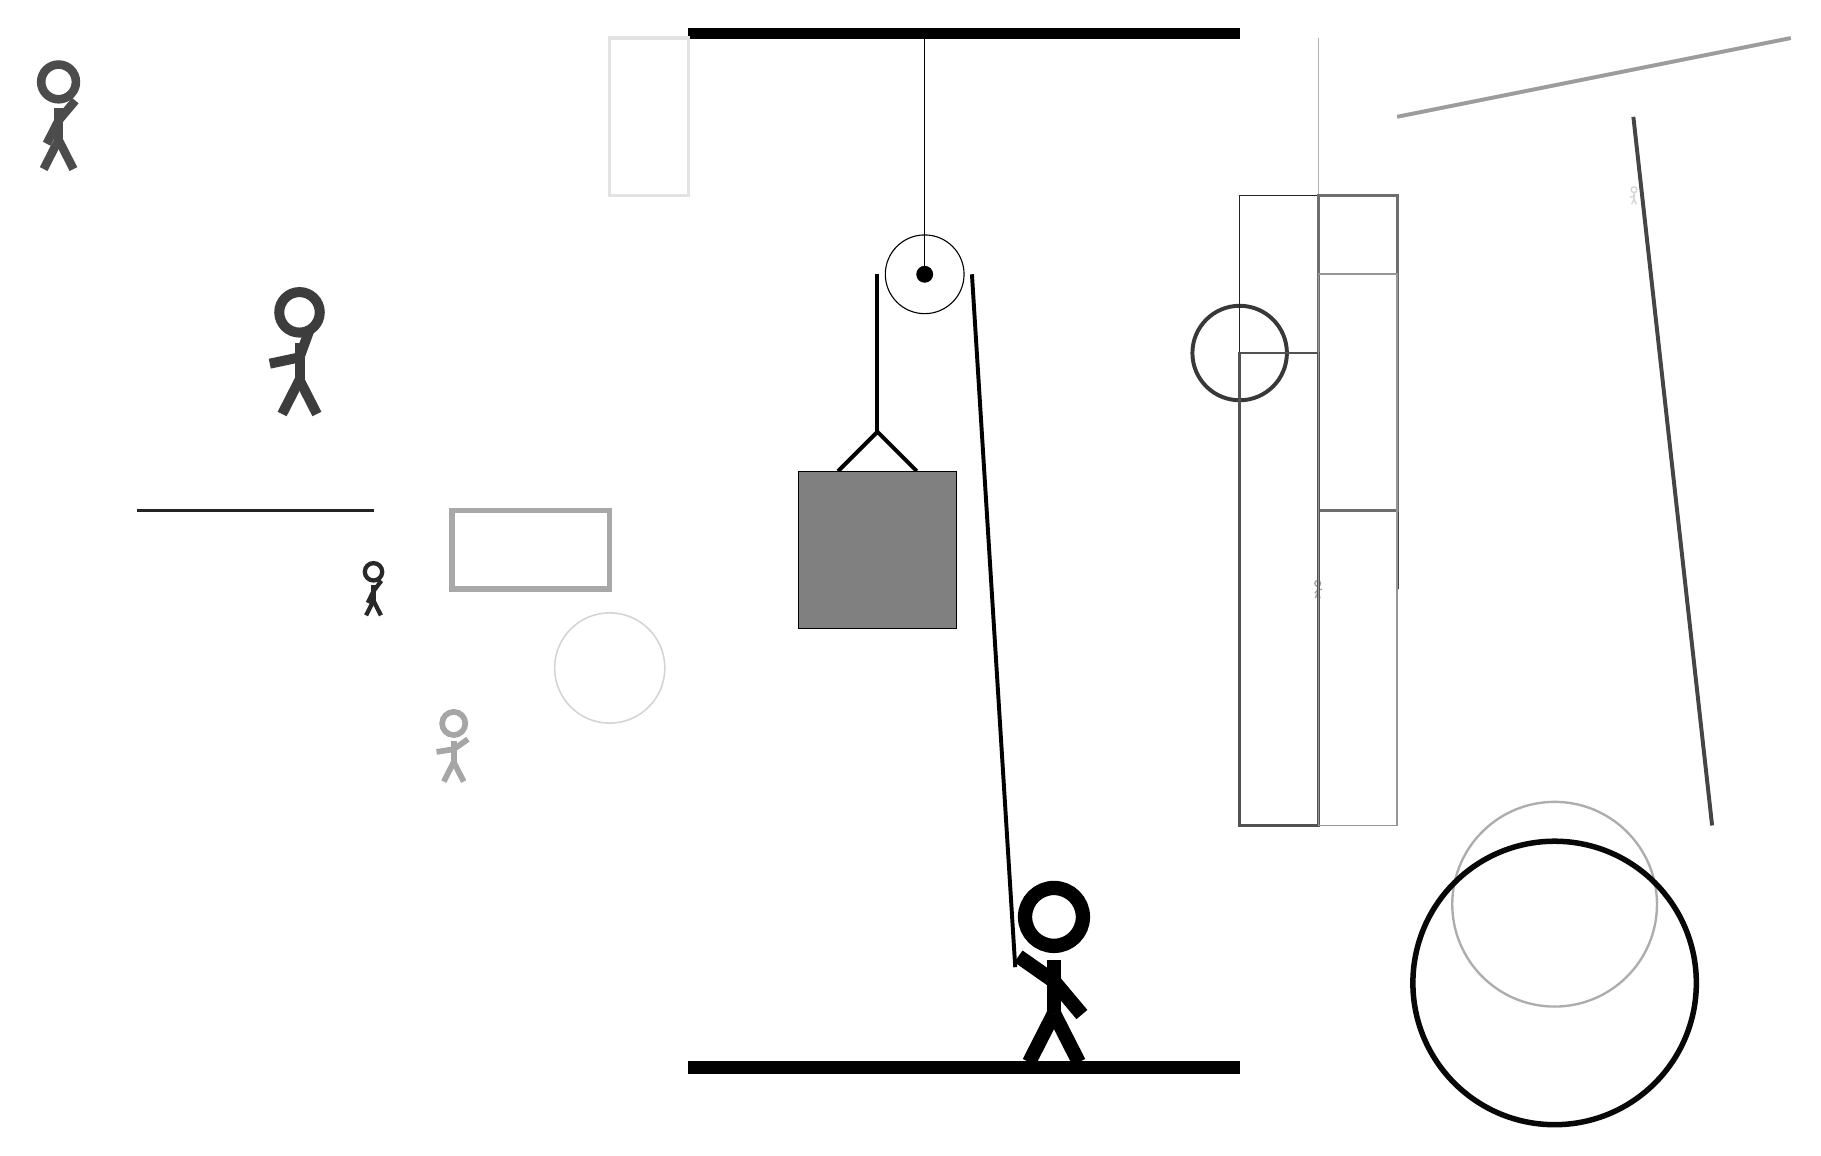
\begin{tikzpicture}
		%%%%% START %%%%%
		
		\draw[fill=black] (-2, 10) rectangle (5, 10.125);
		
		\draw (1, 7) circle (0.5);
		\draw[fill=black] (1, 7) circle (0.1);
		\draw (1, 10) -- (1, 7);
		
		\draw[line width=0.5mm] (-0.1, 4.5) -- (0.4, 5.0) -- (0.9, 4.5);
		\draw[fill=black!50] (-0.6, 4.5) rectangle (1.4, 2.5);
		
		\draw[line width=0.5mm] (0.4, 7) -- (0.4, 5.0);
		\centerarc[line width=0.5mm](1, 7)(0:180:0.6);
		\draw[line width=0.5mm](1.6, 7) -- (2.15, -1.8);
		
		\node[line width=0.5mm, color=black!16] at (10, 8) {\Strichmaxerl[1][14][78]};
		
		\node[line width=0.4mm, color=black!84] at (-6, 3) {\Strichmaxerl[3][64][53]};
		\draw [line width=0.5mm, color=black!78](5, 6) circle (0.6);
		\draw [line width=0.2mm, color=black!17](-3, 2) circle (0.7);
		
		\draw [line width=0.3mm, color=black!32](9, -1) circle (1.3);
		\draw[line width=0.5mm, color=black!39](7, 9) -- (12, 10);
		
		\node[line width=0.2mm, color=black!35] at (-5, 1) {\Strichmaxerl[4][9][35]};
		
		\draw [line width=0.7mm, color=black!97](9, -2) circle (1.8);
		\draw[line width=0.2mm, color=black!31] (6, 8) rectangle (6, 10);
		\draw[line width=0.4mm, color=black!73] (7, 8) rectangle (7, 3);
		
		\draw[line width=0.4mm, color=black!11] (-2, 10) rectangle (-3, 8);
		\draw[line width=0.5mm, color=black!73](10, 9) -- (11, 0);
		\node[line width=0.5mm, color=black!76] at (-7, 6) {\Strichmaxerl[7][12][70]};
		
		\draw[line width=0.7mm, color=black!34] (-3, 3) rectangle (-5, 4);
		\draw[line width=0.2mm, color=black!86] (5, 8) rectangle (6, 0);
		\draw[line width=0.4mm, color=black!57] (7, 8) rectangle (6, 4);
		
		\node[line width=0.4mm, color=black!36] at (6, 3) {\Strichmaxerl[1][51][7]};
		\draw[line width=0.3mm, color=black!68] (5, 6) rectangle (6, 0);
		\node[line width=0.2mm, color=black!70] at (-10, 9) {\Strichmaxerl[6][63][50]};
		\draw[line width=0.2mm, color=black!41] (6, 0) rectangle (7, 7);
		\draw[line width=0.5mm, color=black!86](-6, 4) -- (-9, 4);
		
		
		\node at (2.6, -1.9) {\Strichmaxerl[10][-35][-50]};
		
		\draw[fill=black] (-2, -3) rectangle (5, -3.15);
		
		%%%%% END %%%%%
	\end{tikzpicture}
\end{document}